
\section{Программные средства для моделирования}

Для проведения численных экспериментов было необходимо соответствующее
программное обеспечение. Несмотря на то, что существует значительное количество
программ для моделирования электродинамических задач при помощи метода FDTD,
было решено использовать собственную реализацию, так как доступные открытые
аналоги не устраивали по качеству исполнения, а проприетарные --- тем, что
их рабочие алгоритмы закрыты.

Итак, для моделирования TEM-рупорных антенн, описанного в последующих разделах,
ипользовалась связка из нескольких компьютерных программ, разработанных на
кафедре электроники физического факультета ВГУ. Схема их взаимодействия
представлена на рис.~\ref{fig:Programs:WorkFlow}.

% --- Рисунок
\begin{figure}
\centering
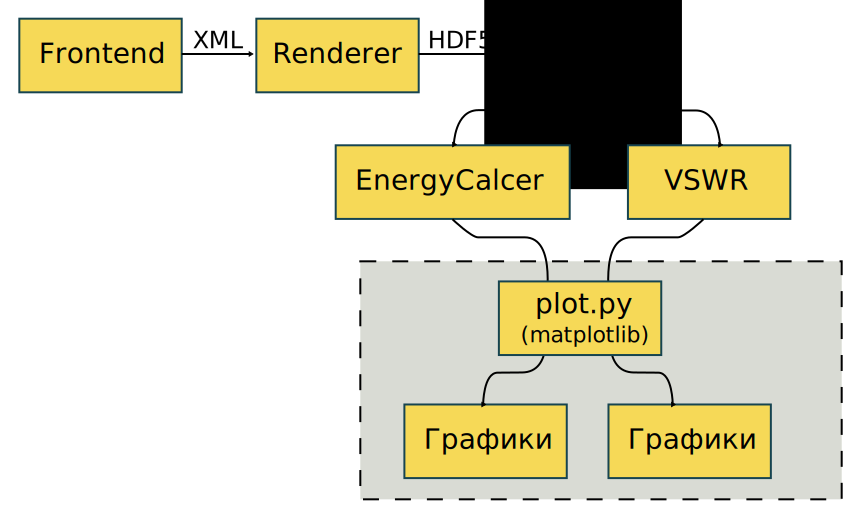
\includegraphics[width=0.7\textwidth]{graphics/programs-work-flow}
\caption{Взаимодействие компонентов программного комплекса моделирования.}
\label{fig:Programs:WorkFlow}
\end{figure}

Функциональное назначение отдельных блоков следующее:
\begin{itemize}
\item Frontend --- редактор трехмерной структуры, подлежащей анализу;
\item Renderer --- формирует трехмерную сетку счетной области, преобразовывая
      структуру из XML-представления, которое является рабочим фоматом
      предыдущей программы, в бинарное представление на основе формата HDF~5,
      удобное для проведения моделирования;
\item Fdtd3d --- расчетный модуль, выполняющий непосредственно моделирование
      и нахождение полей в дальней зоне;
\item EnergyCalcer --- расчитывает энергетические диаграммы направленности,
      используя рассчитанные предыдущей программой поля в дальней зоне;
\item VSWR --- расчитывает коэффициент стоячей волны по напряжению по
      результатам моделирования, полученным программой Fdtd3d;
\item plot.py --- скрипт на языке Python, строящий графики для наглядного
      представления результатов моделирования.
\end{itemize}

Пример работы программы Fdtd Frontend представлен на
рисунках~\ref{fig:Programs:LinearScreenshot}
и~\ref{fig:Programs:ExponentialScreenshot}, полученная в результате
преобразования сетка изображена на
рисунках~\ref{fig:Programs:RenderedLinearScreenshot}
и~\ref{fig:Programs:RenderedLinearScreenshot}. В пункте~\ref{div:FileFormat}
приводится описание бинарного формата данных, связывающего пользовательский
программный модуль с расчетным.

% --- Русонок.
\begin{figure}
\centering
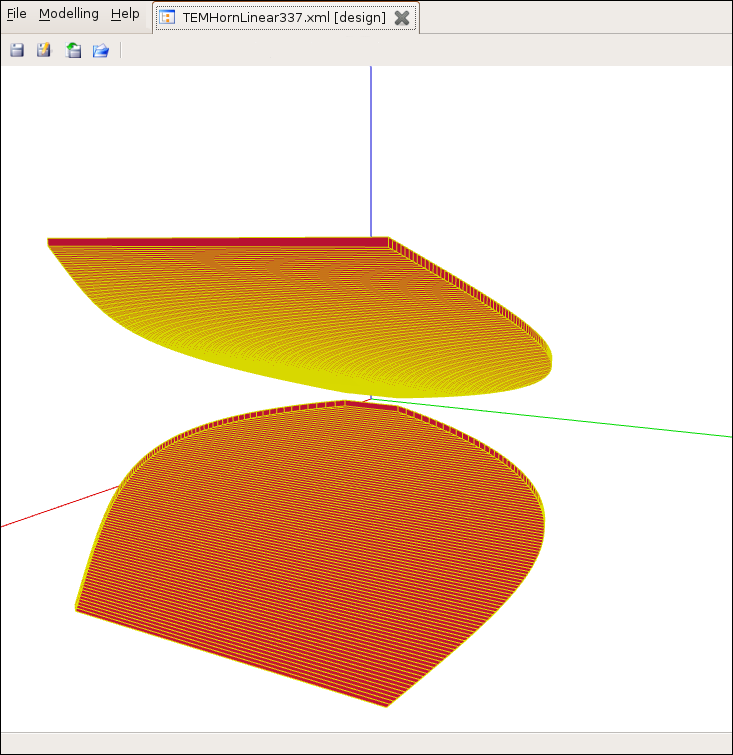
\includegraphics[width=\textwidth]{graphics/screenshot-tem-horn-linear-377}
\caption{
    Пример рабочего окна программы Fdtd Frontend с загруженной антенной
    с линейным профилем раскрыва и выходным волновым
    сопротивлением~$Z_R=\valu{377}{Ом}$.}
\label{fig:Programs:LinearScreenshot}
\end{figure}

% --- Русонок.
\begin{figure}
\centering
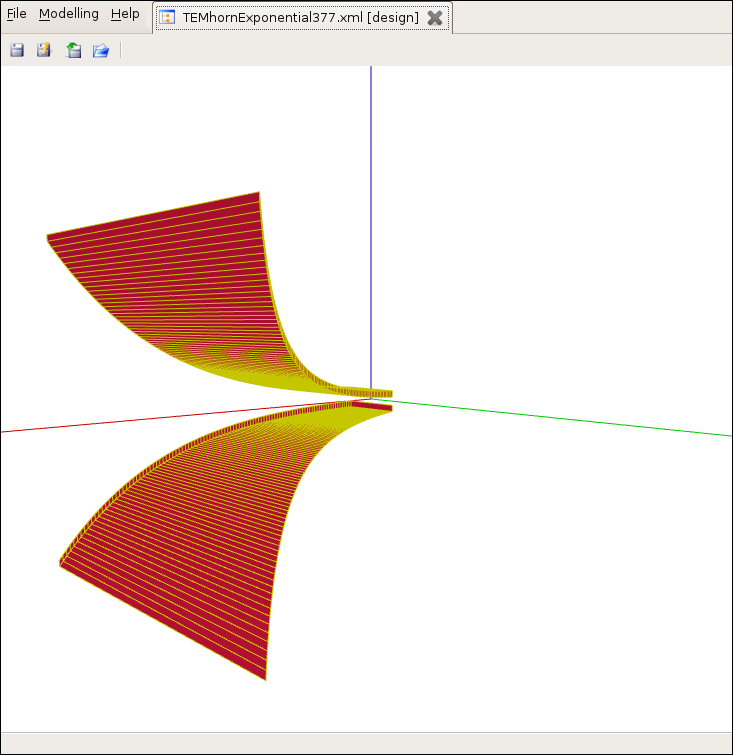
\includegraphics[width=\textwidth]{graphics/screenshot-tem-horn-exponential-377}
\caption{
    Пример рабочего окна программы Fdtd Frontend с загруженной антенной
    с экспоненциальным профилем раскрыва и выходным волновым
    сопротивлением~$Z_R=\valu{377}{Ом}$.}
\label{fig:Programs:ExponentialScreenshot}
\end{figure}

% --- Русонок.
\begin{figure}
\centering
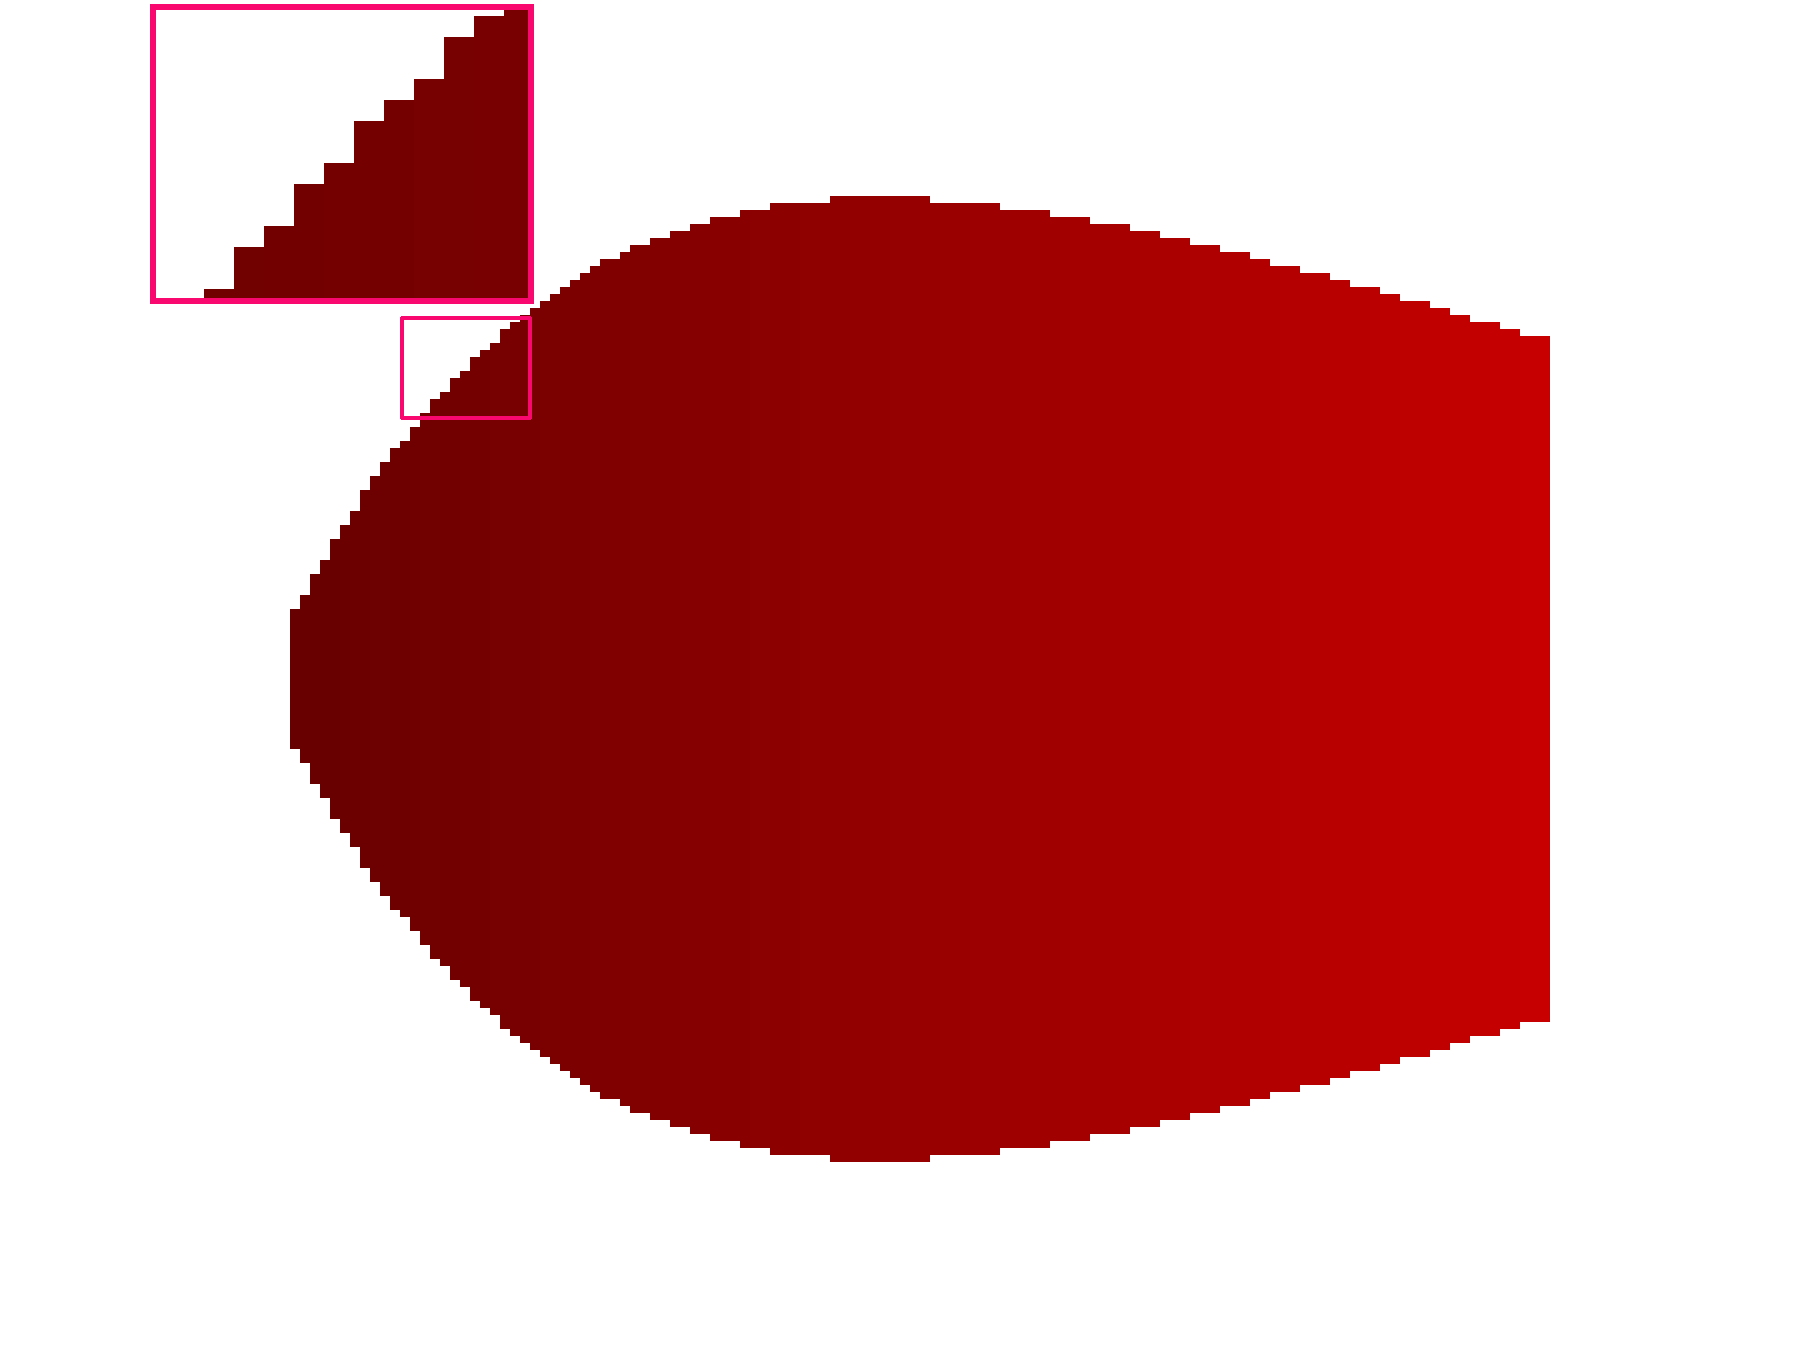
\includegraphics[width=\textwidth]{graphics/screenshot-rendered-linear-377}
\caption{
    Расчетная сетка антенны с линейным профилем раскрыва и выходным волновым
    сопротивлением~$Z_R=\valu{377}{Ом}$, вид сверху.}
\label{fig:Programs:RenderedLinearScreenshot}
\end{figure}

% --- Русонок.
\begin{figure}
\centering

\includegraphics[width=\textwidth]{graphics/screenshot-rendered-exponential-377}
\caption{
    Расчетная сетка антенны с линейным профилем раскрыва и выходным волновым
    сопротивлением~$Z_R=\valu{377}{Ом}$, вид сверху.}
\label{fig:Programs:RenderedExponentialScreenshot}
\end{figure}
